\documentclass{standalone}
\begin{document}
\subsection{Aufgabe 12.8}

a) $\{z \in \mathbb{C} | \: \abs{z+i} \leq 3\}$\\
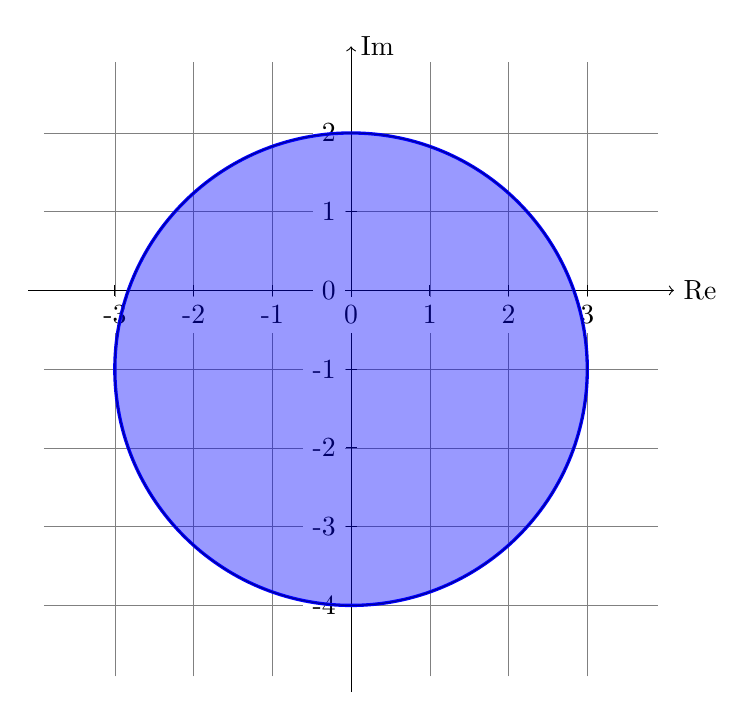
\begin{tikzpicture}
	\draw[very thin, gray] (-3.9, -4.9) grid (3.9, 2.9);
	\draw[->] (-4.1, 0) -- (4.1, 0) node[right]{Re};
	\draw[->] (0, -5.1) -- (0, 3.1) node[right]{Im};
	
	\foreach \x in {-3,...,3}
	\draw (\x, 2pt) -- (\x, -2pt) node[below, fill=white] {\x};
	
	\foreach \y in {-4,...,2}
	\draw (2pt, \y) -- (-2pt, \y) node[left, fill=white] {\y};
	
	\draw[blue, very thick] (0, -1) circle (3);
	\filldraw[fill=blue, opacity=0.4] (0, -1) circle (3);	
\end{tikzpicture}\\

b) $\{z \in \mathbb{C} | \: Re(\bar{z}-i) = z\}$\\
\begin{tikzpicture}
	\draw[very thin, gray] (-2.9, -1.9) grid (2.9, 1.9);
	\draw[->] (0, -2.1) -- (0, 2.1)node[right]{Re};
	\draw[->] (3.5, 0) -- (3.7, 0)node[right]{Im};
	
	\foreach \x in {-2,...,2}
	\draw (\x, 2pt) -- (\x, -2pt) node[below, fill=white] {\x};
	
	\foreach \y in {-1,...,1}
	\draw (2pt, \y) -- (-2pt, \y) node[left, fill=white] {\y};
	
	\draw[dashed] (-3.5, 0) -- (3.5, 0);		
	
	\draw[very thick, red] (-3, 0) -- (3, 0);
	
	\draw[dashed, very thick, red] (-3.5, 0) -- (3.5, 0); 
	
\end{tikzpicture}

\end{document}
